\documentclass[table]{beamer}
\usepackage[utf8]{inputenc}
\usepackage{amsmath}
\usepackage{upgreek}
\usepackage{graphicx}
\usepackage{verbatim}
\usepackage{subcaption}
\usepackage{amsmath}
\usepackage{hyperref}
\usepackage[export]{adjustbox}
\usepackage{calc}
\usepackage{wrapfig}
\usepackage{xcolor}
\usepackage{tikz}
\definecolor{carolinablue}{rgb}{0.6, 0.73, 0.89}

\usetikzlibrary{shadings, patterns, shapes.geometric}


\newcommand\x{\times}
\newcommand\y{\cellcolor{green!10}}
\usetheme{CambridgeUS}
\title[ACO]{Ant Colony Optimization: A New Meta-heuristic}

\author[Dorigo-Caro]{\ Authors:\\ \ \ \ \ \ Marco Dorigo\ \ \ \ \ \ \ \ \ \   Gianni A. Di Caro\\[4mm]Presented by:\\[2mm]Md. Zawad Abdullah (1605002)\\Bishwajit Bhattacharjee (1605003)\\Md. Mahir Shahriyar (1605024)\\[6mm]Department of CSE,\\Bangladesh University of Engineering and Technology }
\date{\today}

\begin{document}
\maketitle


\begin{frame}{Problem Definition}
	\begin{block}{The Traveling Salesman Problem}
		A salesman needs to visit a number of customers located in different cities and return to the starting city using the shortest route.
	\end{block}
\end{frame}


\begin{frame}{Input:}
	\begin{figure}
		\centering
		\def\svgscale{0.9}
		\input{TSPGraph.pdf_tex}
	\end{figure}
\end{frame}


\begin{frame}{Output:}
	\begin{figure}
		\centering
		\def\svgscale{0.9}
		\input{TSPGraphSolution.pdf_tex}
	\end{figure}
\end{frame}

\begin{frame}{Known Methods}
	\begin{itemize}
		\item <1->	Backtracking\\
					\uncover<2->{Issue - Complexity is exponential.}\\
					\uncover<3->{\textbf{Not Good Enough!}}
		\uncover<4->{\item <2->	Bitmask DP\\}
					\uncover<5->{Issue - Works efficiently when input is small.}\\
					\uncover<6->{\textbf{Not Good Enough!}}
	\end{itemize}
\end{frame}


\begin{frame}{Motivation}
	
	\textbf{We will use Ant Colony Optimization (ACO) to solve TSP more efficiently.}
\end{frame}


\begin{frame}{Ants collecting food-1}
	\begin{figure}
		\centering
		\def\svgscale{0.6}
		\input{AntSearch.pdf_tex}
	\end{figure}
	\ \ \ \ \ \ \ \ \ \ \ \ \ \ \ \ \ \ \ \ {\color{blue}Figure:} Paths From Food to Ants' Nest
\end{frame}

\begin{frame}{Ants collecting food-2}
		\begin{figure}
			\centering
			\def\svgscale{0.6}
			\input{AntSearch2.pdf_tex}
		\end{figure}
		\ \ \ \ \ \ \ \ \ \ \ \ \ \ \ \ \ \ \ \ \ \ \ \ \ {\color{blue}Figure:} Ants Searching for Food
\end{frame}


\begin{frame}{Ants collecting food-3}
		\begin{figure}
			\centering
			\def\svgscale{0.6}
			\input{AntSearch3.pdf_tex}
		\end{figure}
		\ \ \ \ \ \ \ \ \ \ \ \ \ \ \ \ \ \ \ \ \ \ \ \ \ {\color{blue}Figure:} Ants Following An Optimal Path
\end{frame}


\begin{frame}
	\centering
	\vspace{\baselineskip}	\vspace{\baselineskip}
	So how do they communicate??\\ 
	{\vspace{\baselineskip}	\vspace{\baselineskip}}
	\uncover<2->{\textcolor{red}{\huge Pheromone}}
	\vspace{\baselineskip}	\vspace{\baselineskip}
	\begin{figure}
		\uncover<3>{\includegraphics[ width=.7\textwidth,left ]{AntPheromone.png}	}
	\end{figure}
\end{frame}

\begin{frame}
	\centering
	\vspace{\baselineskip}	\vspace{\baselineskip}
	So how do they communicate??\\ 
	{\vspace{\baselineskip}	\vspace{\baselineskip}}
	{\textcolor{red}{\huge Pheromone}}
	\vspace{\baselineskip}	\vspace{\baselineskip}
	\begin{figure}
		{\includegraphics[ width=1\textwidth,right ]{AntPheromone3.png}	}
	\end{figure}
\end{frame}


\begin{frame}
	\centering
	\vspace{\baselineskip}	\vspace{\baselineskip}
	So how do they communicate??\\ 
	{\vspace{\baselineskip}	\vspace{\baselineskip}}
	{\textcolor{red}{\huge Pheromone}}
	\vspace{\baselineskip}	\vspace{\baselineskip}
	\begin{figure}
		{\includegraphics[ width=1\textwidth,right ]{AntPheromone2.png}	}
	\end{figure}
\end{frame}


\begin{frame}
	\centering
	\vspace{\baselineskip}	\vspace{\baselineskip}
	So how do they communicate??\\ 
	{\vspace{\baselineskip}	\vspace{\baselineskip}}
	{\textcolor{red}{\huge Pheromone}}
	\vspace{\baselineskip}	\vspace{\baselineskip}
	\begin{figure}
		{\includegraphics[ width=1\textwidth,right ]{AntPheromone3.png}	}
	\end{figure}
\end{frame}





\begin{frame}{Previous Works}
	\begin{columns}
	   	\column{0.5\textwidth}
		\begin{itemize}
			\item In the year 1991, Marco Dorigo proposed an algorithm called "Ant System".
			
%			\item <2-> It was a novel heuristic approach to solve combinatorial optimization problems.
			
			\item  AS was first applied to the Traveling Salesman Problem.
			
%			\item <3-> Later it was extended to a diverse set of optimization problems :
%			Multiple Knapsack(Leguizamón \& Michalewicz), Vehicle routing(Bullnheimer), Graph Coloring(Costa \& Hertz) and so on.
			
		\end{itemize}
	   	\column{0.5\textwidth}
			\begin{figure}[h]
				\centering
				\includegraphics[width=0.7\textwidth]{Dorigo.jpg}
				\caption{Marco Dorigo}
			\end{figure}
	\end{columns}

	
	
\end{frame}

\begin{frame}{Results}
	The ACO meta-heuristic is the result of an effort to define a common framework for all the versions of AS.
\end{frame}

\section{Methods}
\begin{frame}{Notations}
	\begin{itemize}
		\item $ C = \{c_1,c_2,...,c_{N_C} \} $ is a finite set of \textit{components}.
		
		\item $ L = \{l_{c_{i}c_{j}}\ |\ (c_i,c_j)\ \in  \tilde{C}\},\ |L| \leq N^{2}_C $ is a finite set of possible \textit{connections/transitions} among the elements of $ \tilde{C} $, where $ \tilde{C} $ is a subset of the Cartesian product $ C\times C $.
		
		\item $ J_{c_ic_j} \equiv J(l_{c_ic_j}, t) $ is a \emph{connection cost} function associated to each $l_{c_ic_j} \in L $, possibly parameterized by some time measure $t$.
		
		\item $ \psi $ is a \emph{solution} of the problem.
		\item $ J_{\psi}(L,t) $ is a \emph{cost} associated to each solution 	$\psi $.  $ J_{\psi}(L,t) $ is a function of all the costs $ J(c_i,c_j) $ of all the connections belonging to the solution $\psi $ .

	\end{itemize}
\end{frame}

\begin{frame}{Adjacency Matrix}	
	\begin{columns}
		
		\begin{column}{0.6\textwidth}
			\resizebox{\linewidth}{!}{$
				\label{eq:appendrow}
				\left(\begin{array}{cccc}
				\rowcolor{red!20}
				\x  & \x  & \x & \x \\
				0   & \x  & \x & \x \\
				\rowcolor{blue!20}
				0   & 0   & \x & \x \\
				0   & 0   & 0  & \x \\
				\y a  &  b  & \y c &  d\\
				\end{array}\right)
				$}	
		\end{column}
		\begin{column}{0.4\textwidth}
			Here $ A(i,j) $ means row i and col j 
		\end{column}
	\end{columns}
\end{frame}

\begin{frame}{Ant Properties}
	Ants of the colony have the following properties :
	\begin{itemize}
		\item<1-> An ant searches for minimum cost feasible solutions 
		$\hat{\mathnormal{J}}_{\psi} =  \mathnormal{min_{\psi}} \  \hat{\mathnormal{J}}_{\psi}(\mathnormal{L},\mathnormal{t}) $ 
			
		
		\item<2-> An ant k has a memory $ \mathcal{M}^{k} $ that it can use to store
information on the path it followed so far. Memory
can be used to build feasible solutions, to evaluate the
solution found, and to retrace the path backward.

		\item<3-> An ant $ \mathnormal{k} $ located on node $ \mathnormal{i} $ can move to a node $ \mathnormal{j} $ chosen in $ \mathcal{N}_{i}^{k} $. The move is selected applying a probabilistic
		decision rule.
	\end{itemize}
\end{frame}	

\begin{frame}{Ant properties continued...}
     \begin{itemize}
		\item<1-> The ants’ probabilistic decision rule is a function of (i)

		the values stored in a node local data structure $\mathcal{A}_i = [ \mathnormal{{a}_{ij} } ] $ called ant-routing table, obtained by a functional composition of node locally available pheromone trails
		and heuristic values, (ii) the ant’s private memory storing its past history, and (iii) the problem constraints.
		
		\item<2-> When moving from node $i$ to neighbor node $j$ the ant can update the pheromone trail $ \uptau_{ij} $  on the arc $(i, j)$ This is called \emph{online step-by-step pheromone update}.
		
	\end{itemize}
\end{frame}



\begin{frame}{Ant properties continued...}
	\begin{itemize}
		\item<1-> Once built a solution, the ant can retrace the same path
		backward and update the pheromone trails on the traversed arcs. This is called \emph{online delayed pheromone update}.
		
		\item<2-> Once it has built a solution, and, if the case, after it has retraced the path back to the source node, the ant dies, freeing all the allocated resources.
		
	\end{itemize}
\end{frame}

\begin{frame}{How The Method Works}
	\begin{itemize}
		\item<1-> A colony of ants concurrently move through neighbor nodes of $G$
		using information stored in the node-local ant-routing tables. 
		
		\item<2-> By moving, they incrementally build solutions to the problem.
		
		\item<3-> Once an ant has built a solution, it deposits information about 	the quality of the pheromone trails it used.
		
	\end{itemize}
\end{frame}

\begin{frame}{How The Method Works continued...}
	
		Besides ants' activities an ACO algorithm might include too more procedures:
		\newline
	
	\begin{columns}
		\column{0.45\textwidth}
			\begin{block}{Pheromone Trail Evaporation}
				The process by means of which the pheromone trail intensity on the connections automatically decreases over time.
			\end{block}
		\column[]{0.45\textwidth}
			\begin{block}{Daemon Actions}
				Used to implement centralized actions which cannot be performed by single ants.\newline
				
			\end{block}	
	\end{columns}
	
\end{frame}

\begin{frame}{\textbf{procedure} ACO\_meta-heuristic()}
	
	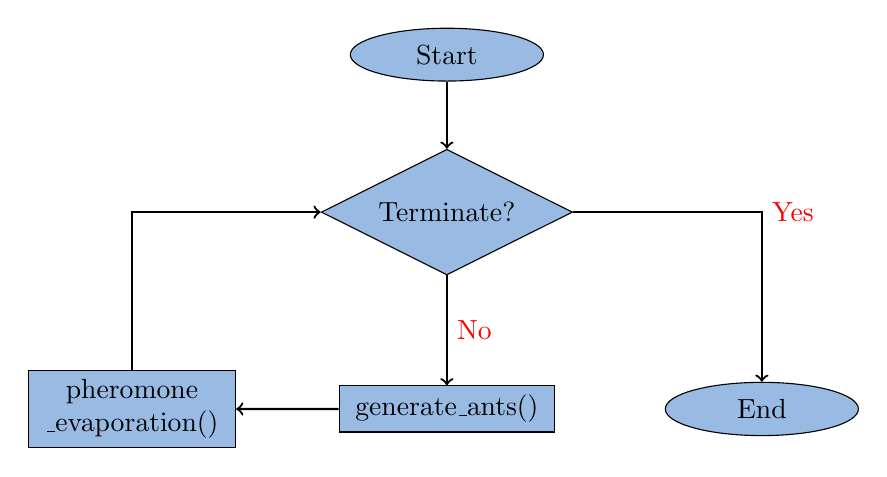
\begin{tikzpicture}
	\node[draw, ellipse, text width = 1.5cm, align=center, yshift=-2cm, fill = carolinablue] (start){Start};
	
	\node[draw, diamond, align=center, below of= start, , text width = 2cm, yshift = -1cm, aspect=2, fill = carolinablue] (cond){Terminate?};
	
	\node[draw, rectangle, align=center, below of= cond, , text width = 2.5cm, yshift = -1.5cm, fill = carolinablue] (activity){generate\_ants()};
	
	\node[draw, rectangle, align=center, left  of= cond, , text width = 2.4cm, xshift = -3cm, yshift=-2.5cm, fill = carolinablue] (eva){pheromone\\\_evaporation()};
	
	\node[draw, ellipse, right of = activity, text width = 1.5cm, xshift = 3cm, align=center, fill = carolinablue] (end){End};
	
	\draw[->, thick] (start) -- (cond);
	
	\draw[->, thick] (cond) -- node[right] {\textcolor{red}{No}} (activity);
	
	\draw[->, thick] (activity) -- (eva);
	
	\draw[->, thick] (eva) |- (cond);
	
	\draw[->, thick] (cond) -| node[right] {\textcolor{red}{Yes}} (end);
	\end{tikzpicture}
\end{frame}

\begin{frame}{\textbf{procedure} generate\_ants()}
	
	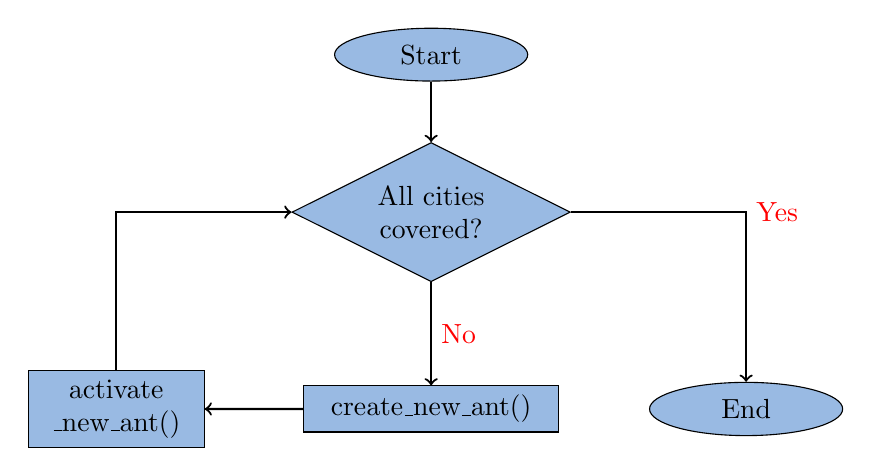
\begin{tikzpicture}
	\node[draw, ellipse, text width = 1.5cm, align=center, yshift=-2cm, fill = carolinablue] (start){Start};
	
	\node[draw, diamond, align=center, below of= start, , text width = 1.5cm, yshift = -1cm, aspect=2, fill = carolinablue] (cond){All cities\\covered?};
	
	\node[draw, rectangle, align=center, below of= cond, , text width = 3cm, yshift = -1.5cm, fill = carolinablue] (creation){create\_new\_ant()};
	
	\node[draw, rectangle, align=center, left  of= cond, text width = 2cm, xshift = -3cm, yshift=-2.5cm, fill = carolinablue] (eva){activate\\\_new\_ant()};
	
	\node[draw, ellipse, right of = creation, text width = 1.5cm, xshift = 3cm, align=center, fill = carolinablue] (end){End};
	
	\draw[->, thick] (start) -- (cond);
	
	\draw[->, thick] (cond) -- node[right] {\textcolor{red}{No}} (creation);
	
	\draw[->, thick] (creation) -- (eva);
	
	\draw[->, thick] (eva) |- (cond);
	
	\draw[->, thick] (cond) -| node[right] {\textcolor{red}{Yes}} (end);
	\end{tikzpicture}
\end{frame}

\begin{frame}{\textbf{procedure} activate\_new\_ant() \{Ant lifecycle\}}
	
	
	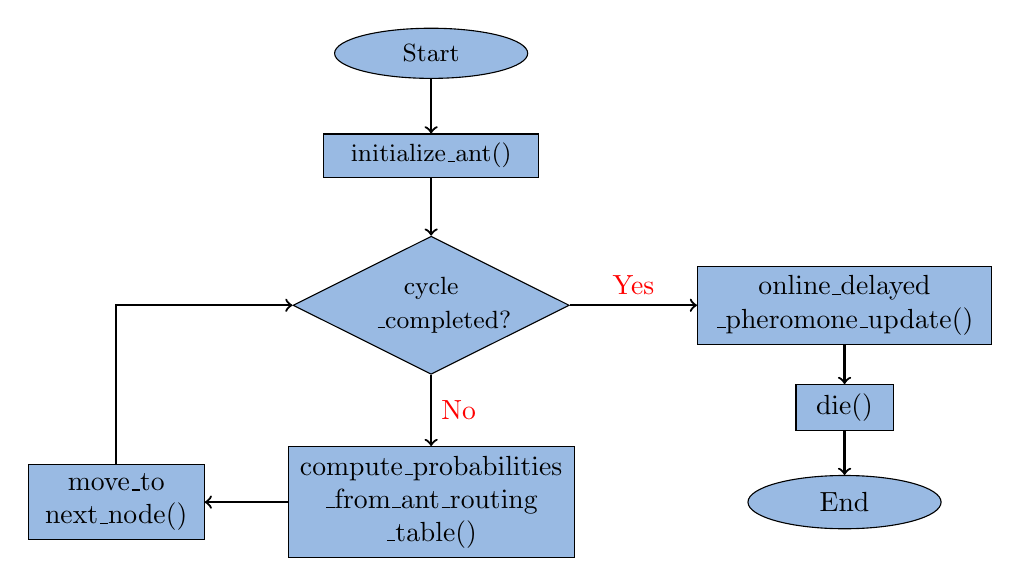
\begin{tikzpicture}
	\node[draw, ellipse, text width = 1.5cm, align=center, fill = carolinablue] (start){\small Start};
	
	\node[draw, rectangle, align=center, below of= start, text width = 2.5cm, yshift = -.3cm, fill = carolinablue] (initialize){\small initialize\_ant()};
	
	\node[draw, diamond, align=center, below of= initialize, text width = 1.4cm, yshift = -.9cm, aspect=2, fill = carolinablue] (cond){\small cycle\\\_completed?};
	
	\node[draw, rectangle, align=center, right of= cond, text width = 3.5cm, xshift=4.25cm, fill = carolinablue] (update){online\_delayed\\\_pheromone\_update()};
	
	\node[draw, rectangle, align=center, below of= cond, , text width = 3.4cm, yshift = -1.5cm, fill = carolinablue] (prob){compute\_probabilities\\\_from\_ant\_routing\\\_table()};
	
	\node[draw, ellipse, right of = prob, text width = 1.5cm, xshift = 4.25cm, align=center, fill = carolinablue] (end){End};
	
	\node[draw, rectangle, align=center, above of= end, text width = 1cm, yshift=.2cm, fill = carolinablue] (die){die()};
	
	\node[draw, rectangle, align=center, left  of= prob, text width = 2cm, xshift = -3cm, fill = carolinablue] (move){move\_to\\next\_node()};
	
	\draw[->, thick] (start) -- (initialize);
	
	\draw[->, thick] (initialize) -- (cond);
	
	\draw[->, thick] (cond) -- node[right] {\textcolor{red}{No}} (prob);
	
	\draw[->, thick] (prob) -- (move);
	
	\draw[->, thick] (move) |- (cond);
	
	\draw[->, thick] (cond) -- node[above] {\textcolor{red}{Yes}} (update);
	
	\draw[->, thick] (update) -- (die);
	
	\draw[->, thick] (die) -- (end);
	\end{tikzpicture}
\end{frame}

\begin{frame}{Traveling Salesman Problem}
	Given a list of cities and the distances between each pair of cities, what is the shortest possible route that visits each city and returns to the origin city?
\end{frame}

\begin{frame}{ACO for the Traveling Salesman Problem}
	
	\begin{itemize}
		\item We construct a graph $G = (C, L) $ where $C$ is the set of components 
			representing cities and $L$ is the set of connections connecting the cities.
		\item $ J_{c_ic_j} $ is the cost of the connection between the nodes $c_i $
		and $ c_j $ , the distance between cities $i$ and $j$ .
		
		\item A solution to this problem is a Hamiltonian circuit with minimal cost.
	\end{itemize}
\end{frame}

\begin{frame}{ACO for the Traveling Salesman Problem Continued}
	
	\begin{itemize}
		\item<1-> A number $m$ of ants are positioned randomly in parallel on $m$ 	cities. Then, they enter a cycle which lasts $ N_C $ iterations.
		
		\item<2-> During each step an ant located on node $i$, reads the entries
		of the ant-routing table. Then it computes the transition probabilities and chooses an adjacent node to move updating it's memory.
		
		\item <3-> Once an ant has completed a tour, it uses its memory to evaluate the built solution. Then it retraces the same tour backward and updates the  pheromone trails of the used edges.	
		
		\item <4-> It uses its memory to avoid visiting a city twice.	
	\end{itemize}
\end{frame}

\begin{frame}{ACO for the Traveling Salesman Problem Continued}
	
	The formula for updating the ant-routing table is:
	
	{\Large $$
		\Large a_{ij} = \frac { {[\uptau_{ij}(t)]}^{\alpha} {[\eta_{ij}]}^{\beta} }
		{\displaystyle\sum_{l \in \mathcal{N}_i} {[\uptau_{il}(t)]}^{\alpha} {[\eta_{il}]}^{\beta} } 
		\ \ \ \ \ \ \ \forall j \in \mathcal{N}_i
		$$}
	
	
	\begin{itemize}
		\item  $ {\uptau_{ij}} $ is the intensity of pheromone trail of the  edge $ 	\mathnormal{l_{ij}} $
		
		\item $ {\eta_{ij}} $ is the heuristic value of the edge between $i$ and $j$.	
		{\Large $$ {\eta_{ij}} = \frac{1}{J_{c_ic_j}} $$ }
		
		\item $\alpha$ and $\beta$ are two parameters that control the relative weight of pheromone trail and heuristic value. 
	\end{itemize}
	
\end{frame}

\begin{frame}{ACO for the Traveling Salesman Problem Continued}
	
	The probability $\mathnormal{p}^{k}_{ij}(t)$ with which an ant $k$ located in city $i$ chooses the city $ j \in \mathcal{N}_i^k $ to move to at the $t$-th  iteration is: 
	
	{\Large 
		$$ \mathnormal{p}^{k}_{ij}(t) = \frac{ {a}_{ij}(t) } 
		{ \displaystyle\sum_{l \in \mathcal{N}_{i}^{k}} a_{il}(t) }
		$$}
	
	where $\mathcal{N}_i^k \subseteq \mathcal{N}_i $ is the feasible neighborhood of node $i$ for ant $k$.
	
\end{frame}

\begin{frame}{ACO for the Traveling Salesman Problem Continued}
	After pheromone updating has been performed by the ants, pheromone evaporation is triggered: the following rule is applied to all the edges $l_{ij}$ of the graph $G$
	
	{\Large
		$$
		\uptau_{ij}(t) \leftarrow (1-\rho)\uptau_{ij}(t)
		$$}\newline
	where $ \rho \in (0,1] $ is the pheromone trail decay coefficient.
\end{frame}

\begin{frame}{Conclusions}
	  In this paper we briefly described ACO and its basic applications. We mainly focused on the use in Traveling Salesman Problem. 
\end{frame}
\end{document}